\chapter{Introdução}
\label{cap:introducao}

A criação dos sistemas de comunicação sem fio revolucionou a forma como a sociedade se conecta e interage com o mundo. Contudo, desde as primeiras redes de transmissão de rádio, um desafio técnico persistente tem acompanhado esse avanço: a interferência eletromagnética entre sinais \cite{kaur2011electromagnetic}. 

% teste

De forma geral, a interferência é qualquer perturbação eletromagnética indesejada que afeta a recepção de um sinal, causada por fontes externas ao sistema receptor, especialmente por outros transmissores operando em frequências próximas ou sobrepostas. Essa perturbação pode degradar o desempenho do sistema ao introduzir ruído, distorção, perda de pacotes ou interrupções na comunicação, comprometendo a confiabilidade e a qualidade do serviço prestado \cite{ott2011electromagnetic}.

Essa problemática é agravada pelo fato de o espectro de radiofrequência ser um recurso físico naturalmente limitado. Embora o espectro eletromagnético se estenda teoricamente por uma faixa infinita de frequências, apenas uma porção específica é viável para aplicações em radiocomunicação. Dentro dessa faixa útil, fatores físicos e tecnológicos impõem restrições adicionais: em baixas frequências, por exemplo, a largura de banda é reduzida e as antenas exigem dimensões elevadas; já em frequências extremamente altas, as ondas se comportam mais como radiação óptica, sofrendo forte atenuação atmosférica, o que limita sua eficácia em aplicações de rádio. Além disso, cada subfaixa só pode suportar um número restrito de transmissões simultâneas exigindo, portanto, um controle rigoroso sobre quem utiliza cada porção do espectro. Na prática, isso significa que a maior parte do espectro útil já está comprometida com algum serviço ou aplicação, configurando o que especialistas chamam de “escassez do espectro” \cite{mitola1999cognitive}. Nesse contexto, a alocação ineficiente de frequências — quando canais são atribuídos de forma subótima a diferentes transmissores — pode levar tanto ao desperdício de recursos quanto a interferências severas, comprometendo a qualidade do serviço e, em casos extremos, inviabilizando completamente a comunicação \cite{viegas2015radios}.

Para evitar o colapso do sistema de comunicações, tornou-se indispensável a implementação de regulamentações governamentais voltadas ao uso racional do espectro eletromagnético, controlando a concessão e o licenciamento das faixas de frequência, além de estabelecer quais serviços podem operar em determinadas bandas, sob condições técnicas específicas e com limites de potência bem definidos \cite{pinheiro2015regulaccao}. Embora a regulamentação seja essencial, ela não resolve por si só o problema técnico da alocação eficiente de frequências em cenários operacionais complexos. Assim, as comunidades científica e técnica passaram a empregar ferramentas da Pesquisa Operacional e da Teoria dos Grafos para modelar matematicamente o problema e buscar soluções algorítmicas que otimizem a distribuição das frequências, reduzam o risco de interferência e façam uso eficiente do espectro disponível \cite{metzger1970spectrum}.

Sob esse cenário, \citeonline{hale1980frequency} apresenta o Problema de Atribuição de Frequências, também chamado de Problema de Atribuição de Canais, que aborda formalmente a questão de como distribuir canais de frequência a transmissores de modo a evitar interferências e satisfazer restrições operacionais. O autor propõe modelar esses problemas por meio de grafos, nos quais os vértices representam os transmissores e as arestas indicam possíveis interferências. Hale discute ainda a equivalência entre certos casos do problema de atribuição e o problema clássico de coloração de vértices em grafos, além de introduzir o conceito de T-coloração, onde vértices adjacentes não podem ter rótulos cuja diferença pertença a um conjunto proibido T (por exemplo, proibindo diferença 0 assegura cores distintas). Essa formulação permitia exigir que transmissores vizinhos não usassem frequências iguais ou até mesmo próximas - por exemplo, evitando que canais adjacentes fossem atribuídos a vizinhos imediatos \cite{LIU1992203, doi:10.1142/S1793830921501032}. Uma resenha \emph{(survey)} sobre T-colorações foi escrita por~\citeonline{roberts1991t}.

Apesar desses avanços, havia  limitações claras. As abordagens anteriores consideravam apenas restrições entre transmissores diretamente adjacentes no grafo (distância 1). Dois transmissores que não fossem vizinhos imediatos (isto é, a distância 2 no grafo) ainda poderiam, na modelagem clássica, receber o mesmo canal, potencialmente causando interferência se estivessem geograficamente próximos (\textit{spillover}). Frederick S. Roberts identificou essa lacuna e, em 1988, em uma comunicação privada aos pesquisadores~\citeonline{griggs1992labelling}, propôs uma generalização do problema de alocação de canais: transmissores “muito próximos” deveriam usar frequências que diferissem mais entre si do que aquelas de transmissores apenas “próximos” (menos próximos). Em termos de grafo, isso significava adicionar uma restrição também para vértices a distância dois, embora mais branda que a restrição entre vizinhos imediatos. Essa ideia visava refletir dois níveis de interferência: um nível forte entre estações vizinhas, e um nível secundário (ainda relevante) entre estações com um intermediário entre elas \cite{franks2015delta2}.

\citeonline{griggs1992labelling}, em resposta à proposta de Roberts, introduziram a Rotulação–L(2,1) que consiste em atribuir inteiros não negativos aos vértices de um grafo de modo que vértices adjacentes recebam rótulos que difiram em módulo de pelo menos duas unidades, e vértices à distância 2 entre si recebam rótulos com diferença mínima de 1. Formalmente, dado um grafo
$G = (V, E)$ simples e não direcionado, uma função $f : V \rightarrow \{0,1,\ldots,k\}$ é dita uma \emph{rotulação–L(2,1)} de $G$ se, para quaisquer dois vértices $u, v \in V$, as seguintes condições forem satisfeitas:

\begin{enumerate}
    \item Se $u$ e $v$ são adjacentes (isto é, $\{u, v\} \in E$), então $|f(u) - f(v)| \geq 2$;
    \item Se $u$ e $v$ estão a distância 2 (isto é, $\text{dist}(u, v) = 2$), então $|f(u) - f(v)| \geq 1$.
\end{enumerate}


\noindent Denominamos por \textit{span} (amplitude)  o maior rótulo atribuído a um vértice do grafo pela função $f$. O \emph{número cromático L(2,1)} de um grafo $G$, denotado por $\lambda(G)$, é o menor \emph{span} atribuído por uma rotulação-L(2,1) de $G$ considerando-se todas as rotulações-L(2,1) possíveis de $G$; ou seja,
\[
\lambda(G) = \min_{f} \left\{ \max_{v \in V} f(v) \right\}.
\] 

\noindent O \emph{Problema da Rotulação-L(2,1)} consiste em determinar o valor exato do parâmetro $\lambda(G)$ para qualquer grafo $G$.

Por exemplo, considere o grafo $G$ ilustrado na Figura~\ref{fig:grafo-exemplo}, no qual cada vértice representa um transmissor e as arestas indicam pares de transmissores com potencial interferência direta. Uma possível rotulação-L(2, 1) é apresentada na Figura~\ref{fig:grafo-com-rotulacao}. Apesar das restrições satisfeitas, essa rotulação apresenta um \emph{span} elevado, evidenciado pela diferença significativa entre os rótulos atribuídos aos vértices extremos $v_1$ e $v_8$. Já a Figura~\ref{fig:grafo-com-rotulacao-otima} exibe uma rotulação–L(2,1) ótima para o mesmo grafo, na qual o valor de $\lambda(G)$ é minimizado respeitando todas as restrições. A comparação entre essas duas soluções reforça a importância da otimização na atribuição de rótulos, especialmente em cenários onde o uso eficiente do espectro é crítico.

\begin{figure}[h]
    \centering
    \caption{Grafo $G$ com oito vértices.}
    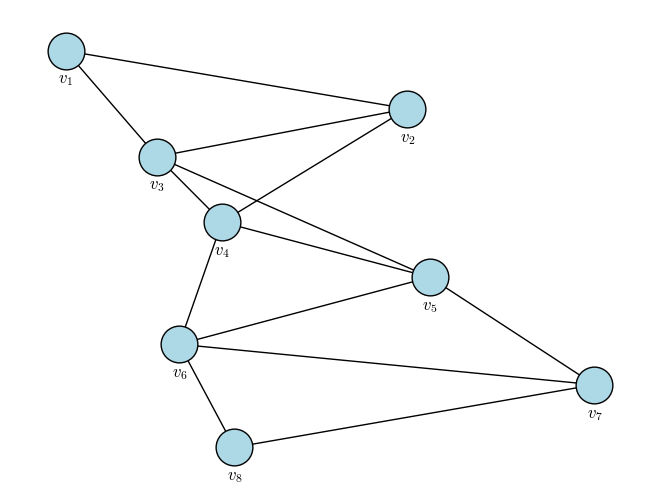
\includegraphics[width=0.6\textwidth]{figuras/grafo exemplo.png}
    \caption*{Fonte: Elaborado pelo autor.}
    \label{fig:grafo-exemplo}
\end{figure}

A rotulação–L(2,1) representa, portanto, um avanço conceitual no tratamento da alocação de frequências, quando comparada à coloração própria de vértices, permitindo modelagens mais alinhadas com os desafios técnicos enfrentados por redes reais. No entanto, resolver esse problema de forma exata é computacionalmente desafiador. Como demonstrado por \citeonline{griggs1992labelling}, a versão de decisão do Problema da Rotulação-L(2,1) é um problema NP-completo.

\begin{figure}[h]
    \centering
    \begin{minipage}[b]{0.48\textwidth}
        \centering
        \caption{Rotulação–L(2,1) de $G$.}
        \includegraphics[width=\textwidth]{figuras/grafo com rotulação.png}
        \caption*{Fonte: Elaborado pelo autor.}
        \label{fig:grafo-com-rotulacao}
    \end{minipage}
    \hfill
    \begin{minipage}[b]{0.48\textwidth}
        \centering
        \caption{Rotulação–L(2,1) ótima.}
        \includegraphics[width=\textwidth]{figuras/grafo com rotulação ótima.png}
        \caption*{Fonte: Elaborado pelo autor.}
        \label{fig:grafo-com-rotulacao-otima}
    \end{minipage}
\end{figure}

A explosão na quantidade de dispositivos e aplicações sem fio evidencia a limitação dos métodos tradicionais de planejamento espectral, os quais se mostram insuficientes, uma vez que  resolver problemas NP-completos de maneira exata torna-se inviável conforme o tamanho da entrada cresce. Isso ocorre, em geral, pois o tempo de execução dos algoritmos exatos cresce de forma exponencial com o tamanho da instância \cite{moscato2001problemas}. Dessa forma, para entradas moderadamente grandes, o tempo necessário para obter uma solução ótima torna-se impraticável, mesmo com computadores modernos. Assim, a complexidade combinatória associada à atribuição de frequências — especialmente sob restrições do tipo L(2,1) — demanda abordagens mais flexíveis e eficientes para encontrar soluções viáveis dentro de prazos computacionais aceitáveis. É nesse contexto que os algoritmos heurísticos ganham destaque \cite{DBLP:journals/corr/abs-1207-1794}.

Algoritmos heurísticos são técnicas de solução que visam encontrar respostas satisfatórias para problemas complexos em tempo computacional reduzido, especialmente quando métodos exatos tornam-se inviáveis devido à elevada complexidade computacional. Em vez de buscar exaustivamente a melhor solução possível, heurísticas exploram o espaço de soluções com base em regras empíricas, estratégias de aproximação ou conhecimento específico sobre a estrutura do problema. Embora não garantam otimalidade nem completude, esses algoritmos oferecem uma alternativa eficiente e prática para lidar com problemas NP-completos, sendo amplamente utilizados em áreas como otimização combinatória, engenharia, inteligência artificial e alocação de recursos em redes de comunicação \cite{pearl1984heuristics}.

Dentre os diversos tipos de algoritmos heurísticos, destacam-se os chamados algoritmos meta-heurísticos, que fornecem estruturas gerais para guiar o processo de busca, muitas vezes inspiradas em fenômenos naturais \cite{Sörensen2013}. Nesse contexto, os algoritmos evolutivos emergem como uma classe particularmente relevante de meta-heurísticas, inspirados nos princípios da evolução biológica, como seleção natural, cruzamento genético e mutação \cite{eiben2015introduction}.

Os \gls{ag} constituem uma das abordagens mais conhecidas e amplamente utilizadas dentro da classe dos algoritmos evolutivos. Inspirados diretamente nos mecanismos de hereditariedade e evolução natural, os \gls{ag}s operam com uma população de soluções, denominadas indivíduos ou cromossomos, que representam possíveis respostas para o problema a ser solucionado. Cada indivíduo é avaliado por meio de uma função de aptidão (\textit{fitness}), que quantifica a qualidade da solução. A partir dessa avaliação, os melhores indivíduos são selecionados para reprodução, onde operadores genéticos, como cruzamento (\textit{crossover}) e mutação, são aplicados com o objetivo de gerar novas soluções, combinando características promissoras de seus “pais” \cite{goldberg1989genetic}.

Ao longo de diversas gerações, espera-se que a população evolua rumo à soluções de qualidade progressivamente melhores, mesmo sem garantia de otimalidade. Essa abordagem baseada em busca estocástica e paralela permite aos \gls{ag}s escapar de mínimos locais e explorar eficientemente espaços de busca complexos e não lineares. Além disso, os \gls{ag}s são altamente flexíveis: podem ser adaptados a diferentes tipos de problemas — contínuos, discretos, com múltiplos objetivos ou com restrições — e facilmente combinados com outras técnicas heurísticas \cite{eiben2015introduction}.

Embora os \gls{ag}s tenham sido amplamente aplicados com sucesso em uma variedade de problemas \cite{faia2018genetic, montana1989training, potvin1996genetic, zhang1997genetic}, sua aplicação ao problema de rotulação–L(2,1) ainda é relativamente pouco explorada na literatura. Os poucos estudos existentes sugerem que os \gls{ag}s têm grande potencial para essa classe de problemas. Isso reforça a necessidade de aprofundar a investigação nessa área. Além disso, as contribuições para a melhor atribuição de frequências podem ter impactos diretos na eficiência e qualidade dos sistemas de comunicação sem fio, promovendo maior acesso à informação, melhor desempenho de redes críticas e suporte à expansão da infraestrutura digital.   

\section{Objetivos}\label{sec:objetivos}
Este trabalho tem como objetivo geral comparar a eficácia de diferentes variações de \gls{ag}s aplicados ao Problema da Rotulação–L(2,1), com foco na minimização do valor $\lambda(G)$ em instâncias de grafos representativos de cenários de interferência em redes de comunicação sem fio. Especificamente, busca-se:

\begin{itemize}

    \item Implementar um algoritmo genético clássico com codificação da solução baseada em ordem e um  algoritmo genético com chaves aleatórias enviesadas para o Problema de Rotulação–L(2,1);
    \item Avaliar o impacto de diferentes parâmetros e operadores genéticos no desempenho dos algoritmos;
    \item Comparar os resultados obtidos em termos de qualidade das soluções (valor de $\lambda(G)$), tempo de execução e estabilidade dos algoritmos com limitantes superiores conhecidos e com uma formulação de programação linear inteira em diferentes classes de grafos.

\end{itemize}

\section{Organização do Projeto}\label{sec:organização-do-trabalho}

Os demais capítulos deste projeto  estão estruturados como a seguir. No Capítulo~\ref{cap:fundamentacao-teorica}, apresenta-se a fundamentação teórica necessária para compreender os principais conceitos envolvidos, abordando a teoria dos grafos, o problema de rotulação–L(2,1), heurísticas clássicas utilizadas nesse contexto, fundamentos sobre \gls{ag}s e suas aplicações em problemas de rotulação. O Capítulo~\ref{cap:trabalhos-relacionados} reúne trabalhos relacionados que exploram abordagens heurísticas e evolucionárias para o problema, com destaque para estratégias que influenciaram a proposta deste estudo. O Capítulo~\ref{chap:metodologia} descreve a metodologia adotada no decorrer desta pesquisa. Por fim, o Capítulo~\ref{cap:resultados} apresenta os resultados preliminares obtidos até o momento.